\chapter{Stima della \textit{body composition} con metodi automatici ed effetti del mezzo di contrasto}
Dopo aver esposto, nel capitolo \ref{capitolo2}, quali sono gli ambiti di interesse della segmentazione di alcuni tessuti corporei attraverso immagini TC, il presente lavoro di tesi ha come obiettivo quello di fare il punto sullo stato dell'arte della segmentazione automatica delle immagini TC per le strutture utili alla \textit{body composition}. Il presente capitolo, dunque, si articola in tre paragrafi: nel primo paragrafo viene svolto un discorso generale sulla segmentazione automatica di immagini TC mediante i risultati riportati in diversi articoli; il secondo tratta gli effetti che il mezzo di contrasto può avere sulle grandezze \textit{CT-derived}, e su come i software di segmentazione automatica e semiautomatica rispondono a questi effetti; infine, nel terzo ci si sofferma sui vantaggi dei metodi di segmentazione 3D.

\section{Stato dell'arte sulla segmentazione automatica dei tessuti corporei attraverso immagini TC}
Uno degli studi più recenti in questo ambito è quello svolto da Borrelli \textit{et al.} \cite{Borrelli2021}, in cui il software di segmentazione, basato su una rete neurale a convoluzione (CNN, di cui si tratta nel paragrafo \ref{retineurali}), è stato allenato su un \textit{training set} costituito da 50 scansioni TC ottenute da una coorte di 50 pazienti affetti da linfoma, con \textit{slice} dallo spessore di 3\,mm; il software è stato poi testato su \textit{test set} di 148 TC ottenute da un gruppo di 74 pazienti colpiti da tumore alla prostata, con \textit{slice} dallo spessore di 5\,mm. Entrambi i gruppi di scansioni sono stati acquisiti mediante un sistema integrato PET/TC. Le immagini TC del \textit{training set} sono state segmentate da uno specialista di medicina nucleare, limitatamente però al tessuto adiposo sottocutaneo (SAT) e al tessuto muscolare, escludendo quindi il tessuto adiposo viscerale (VAT). Sono stati così calcolati i volumi di SAT e muscolo dalla vertebra T11 fino alla zona caudale dell'osso iliaco; sono stati identificati come SAT i voxel (corrispettivo volumetrico del pixel) con HU compreso tra $-190$ e $-30$, come muscolo i voxel con HU compreso tra $-30$ e 150. Per il \textit{test set} è stata eseguita una segmentazione manuale su una sola \textit{slice} per acquisizione all'altezza della vertebra L3, usando gli stessi intervalli della scala Hounsfield di prima. Il software di segmentazione automatica utilizzato (sviluppato da RECOMIA, disponibile online e completamente gratuito \cite{recomia}) assegna a ogni pixel un valore da 0 a 1 e il singolo pixel viene poi assegnato alla categoria in cui ha ottenuto il punteggio più alto. Per valutare l’accuratezza della segmentazione effettuata dal software viene utilizzato il coefficiente di similarità di Dice, impiegato in questo specifico caso per calcolare la sovrapposizione tra le segmentazioni automatica e manuale in una singola \textit{slice} all'altezza della vertebra L3.
Dati due insiemi \textit{X} e \textit{Y}, il coefficiente di Dice è definito come:
\begin{equation}
    DC = \dfrac{2\,\abs{X \cap Y}}{\abs{X}+\abs{Y}}\,,
\end{equation}
dove $\abs{X}$ e $\abs{Y}$ sono le cardinalità dei due insiemi, cioè il numero di elementi di ciascun insieme \cite{dice}.

Tornando a quanto riportato in \cite{Borrelli2021}, il coefficiente di Dice medio per il \textit{test set} è risultato essere 0,96 per il SAT e 0,94 per il tessuto muscolare, indice di un ottimo accordo fra le segmentazioni manuale e automatica, di cui un esempio è presentato nella \figref{fig:borrelli_segmentazione}. Poiché il \textit{test set} era composto da due TC per ogni paziente, eseguite in media a tre giorni di distanza l’una dall'altra, è stata calcolata anche la riproducibilità della segmentazione automatica, che è risultata essere decisamente maggiore per i volumi piuttosto che per le singole \textit{slice}. La differenze relative fra i due studi sono risultate essere di 1,8\% e 5\% rispettivamente per i volumi e le superfici di SAT e di 1,9\% e 3,9\% rispettivamente per i volumi e le superfici di tessuto muscolare.
\begin{figure}[htp]
\centering
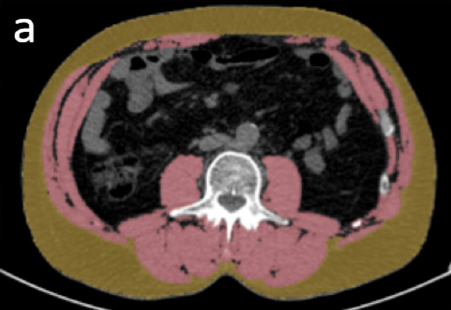
\includegraphics[scale=0.806]{Immagini/borrelli_manual.png}\quad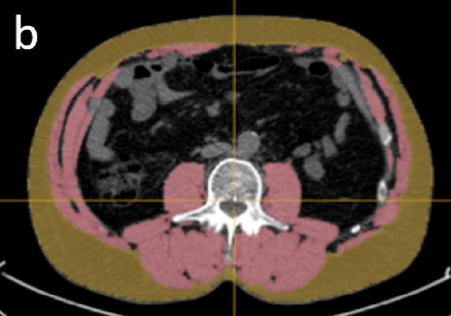
\includegraphics[scale=0.791]{Immagini/borrelli_ai.png}
\caption{\label{fig:borrelli_segmentazione} \textit{Segmentazione manuale (a) e automatica (b) di SAT (in marrone) e muscolo (in rosa) di una slice TC ad altezza L3. Fonte:} \cite{Borrelli2021}.}
\end{figure}

Un punto molto importante presente in \cite{Borrelli2021} è l'elaborazione di due modelli di regressione lineare, riportati nella \figref{fig:borrelli_regressione}, per predire i volumi dei tessuti a partire dalle superfici alla vertebra L3. Per il SAT, l’equazione della retta di regressione è $ y = 35,63\,x + 630,3 $, con un coefficiente di correlazione lineare $ r^2 = 0,83 $. Per il tessuto muscolare il modello è dato dall'equazione $ y = 40,15\,x + 1461 $, con $ r^2 = 0,64 $. Tutte le argomentazioni sopra riportate indicano una netta convenienza nell'utilizzare i volumi di SAT e muscolo piuttosto che le superfici a L3. Infine, nello studio viene messa in luce una limitazione del software di RECOMIA, in particolare dovuta al fatto che nel 9\% dei casi si sia reso necessario l’intervento di un radiologo per correggere la segmentazione proposta dal software stesso. Un’altra importante limitazione, assolutamente non banale, è il fatto che non sia stato preso in considerazione il VAT, assolutamente indispensabile nella formulazione, ad esempio, di un piano terapeutico.
\begin{figure}[htp]
\centering
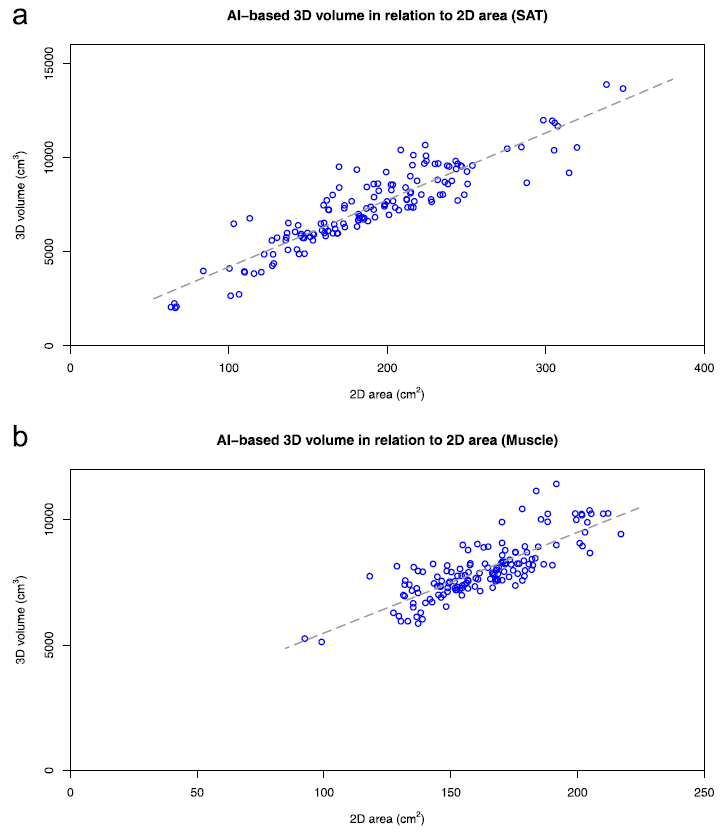
\includegraphics[scale=1]{Immagini/borrelli_regressione.png}
\caption{\label{fig:borrelli_regressione} \textit{Grafico di correlazione tra volumi e superfici di SAT (a) e muscolo (b) calcolati da segmentazione automatica di slice TC ad altezza L3. Fonte:} \cite{Borrelli2021}.}
\end{figure}

Uno studio su una coorte più ampia e differenziata è stato eseguito da Magudia \textit{et al.} \cite{Magudia2021}; anche questo lavoro ha lo scopo di dimostrare la validità della segmentazione automatica, effettuata con una U-Net, per il calcolo della composizione corporea, sempre mediante misurazioni effettuate a livello della vertebra L3, poiché queste sono ben correlate, solitamente, con SAT, VAT e muscolo scheletrico (SM) totali (in tutto il corpo). Il \textit{data set} di questo studio è costituito da 604 TC addominali, una per ogni paziente, tutti affetti da adenocarcinoma pancreatico: 421 TC sono state usate per l’allenamento, 94 per la validazione%
\footnote{Un \textit{data set} di validazione è un insieme di dati \virgolette{ibrido}, in quanto si tratta di un \textit{data set} considerato ancora di allenamento ma che viene utilizzato per testare l’apprendimento del software; tuttavia, non prende parte né nel processo di allenamento di basso livello né nella fase di \textit{testing} finale \cite{sets}.}
e 89 per il \textit{testing} del modello finale. I pazienti sono per il 49\% uomini e per il 51\% donne, con un’età media di 54 anni. È stato utilizzato anche un secondo, esterno \textit{test set} costituito da 534 TC addominali di pazienti colpiti da linfoma. Per la segmentazione manuale del \textit{training set} sono stati utilizzati gli stessi valori di HU dello studio precedente \cite[vedi][]{Borrelli2021}. La coorte su cui il software è stato impiegato è di 12128 membri, selezionati tra pazienti senza comorbidità oncologiche o cardiovascolari note, in modo da rendere lo studio rappresentativo della popolazione generale. Le associazioni tra le CSA dei diversi tessuti e parametri come età, sesso e razza sono state determinate con test di Student e regressioni lineari. Dall’SMI è stato trovato che il 35\% dei pazienti manifestava sarcopenia, diagnosticata per SMI inferiore a 55\,$\mathrm{cm}^2/\mathrm{m}^2$ per gli uomini e 39\,$\mathrm{cm}^2/\mathrm{m}^2$ per le donne. I coefficienti di Dice per SM, SAT e VAT sono stati calcolati rispettivamente in $0,97\pm0,03$, $0,98\pm0,02$ e $0,95\pm0,10$; l'accuratezza delle segmentazione automatica è constatabile, oltre che dai coefficienti di Dice, anche dall'esempio riportato nella \figref{fig:magudia_segmentazione}.
\begin{figure}[t]
\centering
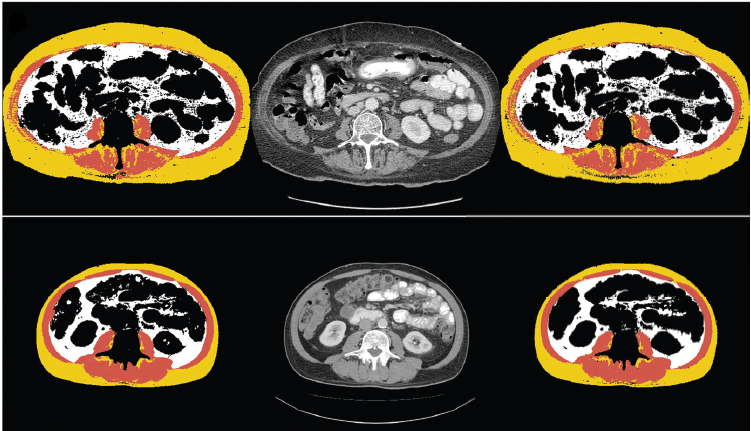
\includegraphics[scale=0.99]{Immagini/magudia_segmentazione.png}
\caption{\label{fig:magudia_segmentazione} \textit{Slice TC ad altezza L3 (al centro) e loro segmentazioni automatiche (a sinistra) e manuali (a destra). Il muscolo scheletrico è evidenziato in marrone, il grasso sottocutaneo in giallo e il grasso viscerale in bianco, mentre tutto il resto è riportato in nero. Fonte:} \cite{Magudia2021}.}
\end{figure}
Sono state calcolate curve di riferimento sia per le CSA di ciascuna tipologia di tessuto sia per i loro indici (vale a dire le superfici di ciascun tessuto divise per l’altezza al quadrato di ciascun paziente) in funzione di età, sesso e razza. Come ci si aspettava, sono state trovate CSA maggiori di SM e VAT e CSA lievemente minori di SAT negli uomini rispetto alle donne. Altri risultati sono l’aumento generale di VAT con l’aumentare dell'età e allo stesso tempo la perdita di SM, come riportato nei grafici di \figref{fig:magudia_smvat}. La CSA di SM è più o meno simile confrontando pazienti bianchi e pazienti neri, mentre i pazienti neri dimostrano valori di VAT generalmente più bassi dei bianchi. In ogni caso, il fatto più interessante è proprio che le curve di riferimento attestino differenze fra i gruppi etnici nella composizione corporea, cosa che invece non si riesce a dimostrare utilizzando il peso o l’indice di massa corporea.
\begin{figure}[htp]
\centering
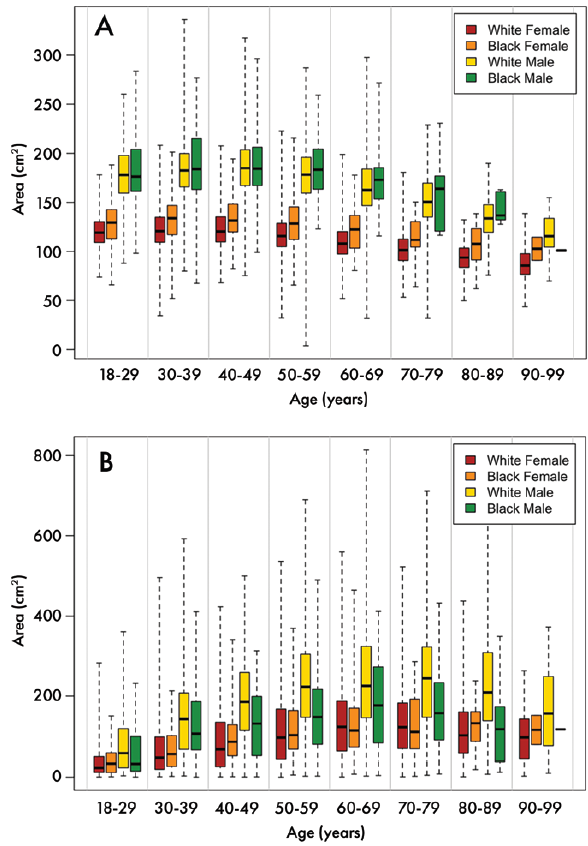
\includegraphics[scale=0.95]{Immagini/magudia_smvat.png}
\caption{\label{fig:magudia_smvat} \textit{Grafici delle CSA di muscolo scheletrico (A) e grasso viscerale (B), con popolazione divisa per sesso e razza. Fonte:} \cite{Magudia2021}.}
\end{figure}

In \cite{Hemke2020} viene testata una rete neurale a convoluzione per la segmentazione automatica dei tessuti corporei, non come al solito all'altezza di L3 ma nella regione pelvica. Il \textit{data set} è costituito da TC addominali di 200 pazienti, di cui 180 sono state utilizzate per l’allenamento e 20 per testare la CNN. Questo lavoro si distingue dagli altri perché tiene in considerazione ben 6 regioni diverse: oltre ai pixel di sfondo, vengono classificati SAT, muscolo, tessuto adiposo intermuscolare (IMAT), osso e tutto il rimanente contenuto intrapelvico (viscere e VAT). I risultati ottenuti nel calcolo della massa muscolare sono comparabili con quelli di altri lavori eseguiti con metodi automatici all'altezza delle vertebre L3 e L4. L’importanza dello studio della regione pelvica sta nell'associazione di alcuni disordini neuromuscolari con infiltrazioni adipose e atrofia della regione pelvica. Sebbene il volume muscolare \textit{total body} sia fortemente correlato con \textit{slice} trasversali della regione L3-L4, misure del grado di sarcopenia a quell'altezza possono essere anche molto diverse da misure effettuate su altre vertebre. Questo elemento può generare valutazioni errate se viene presa in considerazione solamente la regione L3-L4: ad esempio, la massa muscolare della regione pelvica, funzionalmente molto importante per la motilità degli arti inferiori, è di solito maggiore rispetto alla massa muscolare di L3-L4. I coefficienti di Dice per le varie regioni sono riportati in \tabref{tab:dice}; i valori trovati sono comparabili con quelli ottenuti all'altezza di L3 negli altri studi presentati precedentemente. Un esempio dell'accuratezza della CNN impiegata è riportato nella \figref{fig:hemke_segmentazione}; d'altra parte il software ha mostrato difficoltà nel distinguere regioni di confine, come quelle tra muscoli e viscere (\figref{fig:hemke_viscere}) e lungo la fascia muscolare addominale (\figref{fig:hemke_fascia}).
\begin{table}[htp]
    \centering
    \begin{tabular}{|c|c|}
        \hline
        \textit{Label}                      & Coefficiente di Dice  \\ \hline
        Sfondo                              & 1                     \\
        Tessuto adiposo sottocutaneo        & 0,97                  \\
        Tessuto muscolare                   & 0,95                  \\
        Tessuto adiposo intermuscolare      & 0,91                  \\
        Tessuto osseo                       & 0,92                  \\
        Tessuto adiposo viscerale e viscere & 0,98                  \\ \hline
    \end{tabular}
    \caption{\textit{Coefficienti di Dice per tessuto da immagini TC della regione pelvica}.}
    \label{tab:dice}
\end{table}

\begin{figure}[htp]
\centering
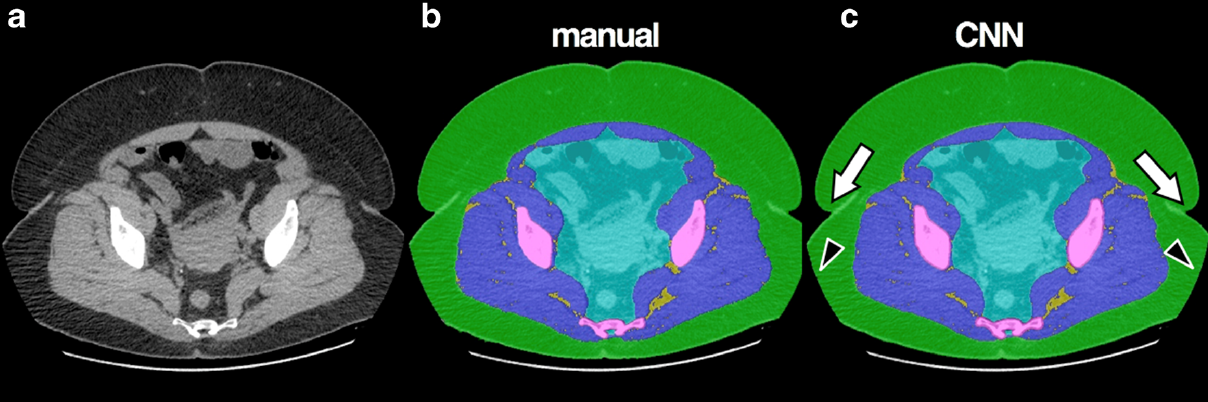
\includegraphics[scale=0.615]{Immagini/hemke_segmentazione.png}
\caption{\label{fig:hemke_segmentazione} \textit{Immagine TC (a) e sue segmentazioni manuale (b) e automatica (c), caratterizzata da una quantità elevata di SAT. Ai tessuti sono assegnati seguenti colori: verde per il SAT, giallo per l'IMAT, magenta per l'osso, blu per il muscolo e azzurro per le viscere e il VAT. La CNN ha dimostrato un buon comportamento anche in situazioni non scontate, come nel riconoscere le pieghe della pelle (freccia bianca) e il cut-off del campo visivo della scansione (freccia nera). Fonte:} \cite{Hemke2020}.}
\end{figure}
\begin{figure}[htp]
\centering
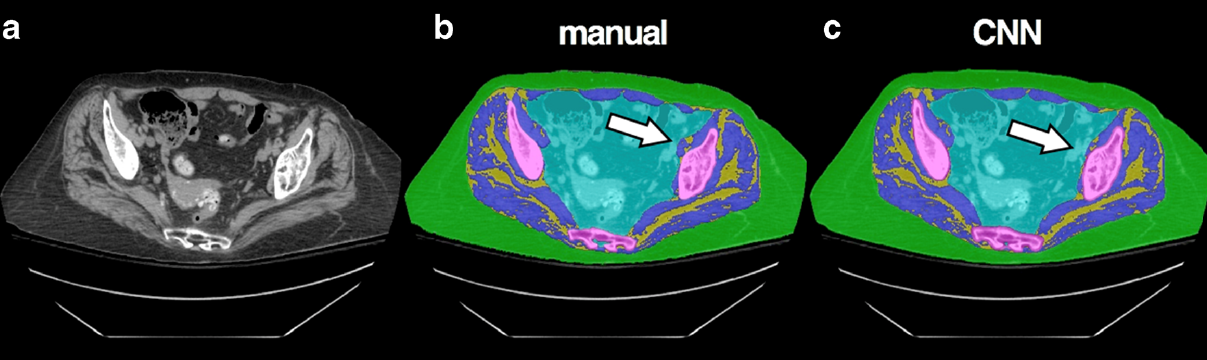
\includegraphics[scale=0.615]{Immagini/hemke_viscere.png}
\caption{\label{fig:hemke_viscere} \textit{Immagine TC (a) e sue segmentazioni manuale (b) e automatica (c), caratterizzata da una quantità elevata di IMAT. La freccia bianca indica una piccola porzione di tessuto che la CNN riconosce come viscere, mentre in realtà si tratta di muscolo. Fonte:} \cite{Hemke2020}.}
\end{figure}
\begin{figure}[htp]
\centering
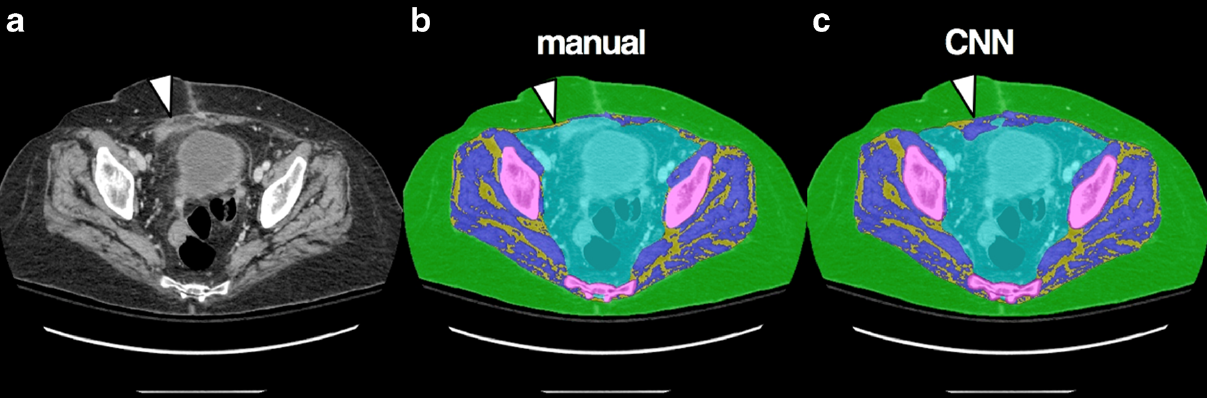
\includegraphics[scale=0.615]{Immagini/hemke_fascia.png}
\caption{\label{fig:hemke_fascia} \textit{Immagine TC (a) e sue segmentazioni manuale (b) e automatica (c). La freccia bianca indica una piccola porzione di tessuto che la CNN riconosce come muscolo, mentre in realtà si tratta di tessuto viscerale misto e grasso viscerale. Fonte:} \cite{Hemke2020}.}
\end{figure}

\section{Effetti del mezzo di contrasto sulle grandezze \textit{CT-derived}}
I mezzi di contrasto sono sostanze che vengono somministrate ai pazienti prima o durante un qualche esame diagnostico (TC, \textit{imaging} di risonanza magnetica, esami con ultrasuoni) per permettere al radiologo di evidenziare condizioni patologiche all'interno di un’immagine e, in generale, di migliorare la qualità dell'immagine, aumentando il contrasto fra una regione del corpo e le regioni circostanti. Un mezzo di contrasto può essere somministrato per via orale, rettale o intravenosa. Per la TC e le immagini radiologiche in generale, il mezzo di contrasto può essere una soluzione a base di iodio, immessa nel corpo per via endovenosa o in cavità varie, oppure un composto a base di solfato di bario, somministrato in questo caso per via orale in diverse forme \cite{contrast}. L’effetto del mezzo di contrasto si esprime in un cambio del coefficiente di attenuazione lineare dei tessuti, quindi in un cambio di valori all'interno della scala Hounsfield. Questo rappresenta un problema per un algoritmo di segmentazione, che viene calibrato in base a certi valori di HU per ciascun tipo di tessuto, e che di conseguenza potrebbe fallire nel caso in cui le immagini da analizzare siano influenzate dal mezzo di contrasto. Diventa importante, di conseguenza, indagare come cambiano i valori di HU quando al paziente viene somministrato un mezzo di contrasto.

Per cominciare, uno studio di Fuchs \textit{et al.} \cite{Fuchs2018} ha investigato l’effetto del mezzo di contrasto intravenoso (IV) sulle misure di superficie (\textit{cross sectional skeletal muscle area}, CSMA) e densità (\textit{skeletal muscle density}, SMD) del tessuto muscolare scheletrico, all'interno di un esame angiografico eseguito mediante TC (\textit{computed tomography angiography}, CTA). Le misure di CSMA e SMD sono state eseguite a livello della vertebra L3, su un \textit{data set} costituito da 114 immagini estratte da 38 CTA. La soglia di definizione del muscolo scheletrico è stata definita, come al solito, tra $-29$ e 150\,HU, mentre la SMD è stata definita come l’attenuazione media della superficie di muscolo segmentata. I valori di CSMA e SMD sono stati registrati su ciascun paziente durante la stessa indagine diagnostica e confrontati con altre serie di valori acquisiti durante la stessa indagine variando specifici parametri tecnici; il confronto fra le serie di dati è stato effettuato mediante il metodo Bland-Altman, presentato nel paragrafo \ref{blandaltman}. La segmentazione è stata effettuata con un software semiautomatico. Confrontando le superfici misurate su \textit{slice} spesse 2\,mm con e senza mezzo di contrasto, sono stati rilevati valori di CSMA significativamente più alti nel primo caso rispetto al secondo: in una media su tutti i pazienti, la superficie trasversale è risultata maggiore dell'1,88\%; lo stesso vale per l’SMD, più grande del 5,99\% nelle immagini con mezzo di contrasto rispetto a quelle senza.

Nello stesso studio, su un altro \textit{data set} costituito da 102 immagini estratte da 38 PET/TC (senza mezzo di contrasto), sono state svolte analisi sulle dipendenze di CSMA e SMD dallo spessore delle \textit{slice} e dalla corrente del tubo a raggi X. Tralasciando il secondo punto, che richiederebbe una discussione che esula dallo scopo di questa tesi, sono stati trovati dati interessanti riguardo allo spessore delle \textit{slice}: è stato rilevato un aumento medio dell'1,11\% della CSMA all'altezza di L3 se si impiega una \textit{slice} dello spessore di 5\,mm rispetto a una dello spessore di 2\,mm; parallelamente, i valori di SMD sono minori dell'11,64\% per i 5\,mm rispetto ai 2\,mm. Nella \figref{fig:fuchs_ba} sono riportati i grafici di Bland-Altman riguardanti le dipendenze di CSMA e SMD appena esposte.
\begin{figure}[H]
\centering
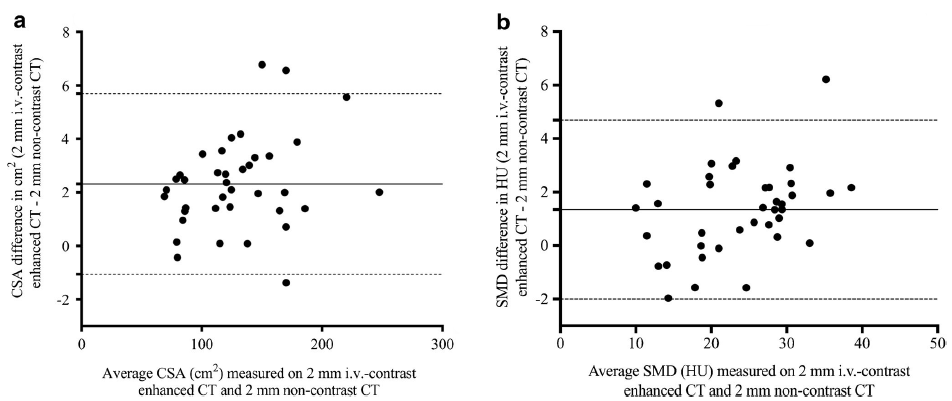
\includegraphics[scale=0.78]{Immagini/fuchs_contrasto.png}\quad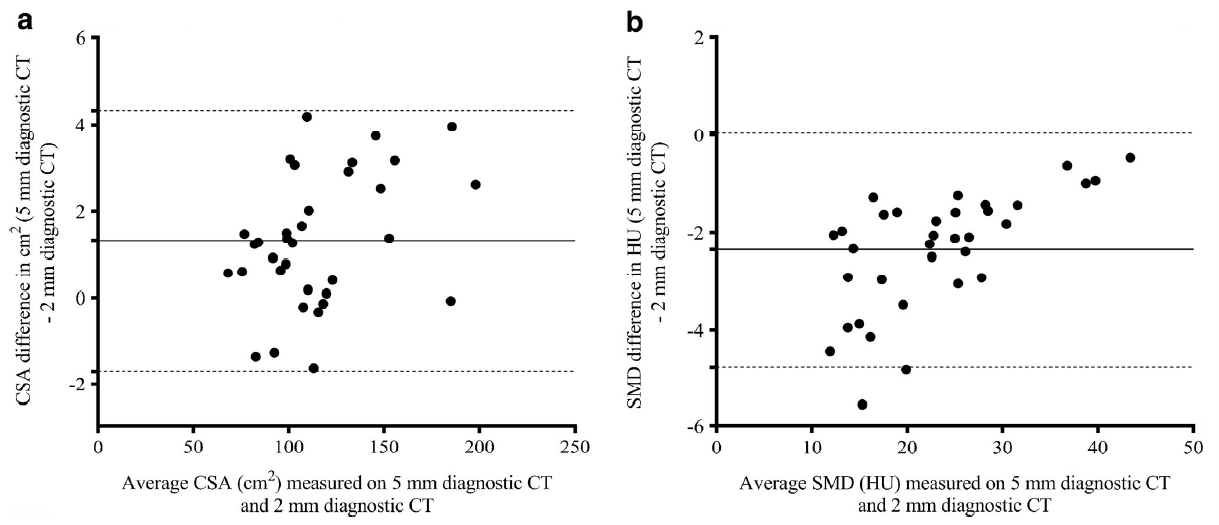
\includegraphics[scale=0.61]{Immagini/fuchs_spessore.png}
\caption{\label{fig:fuchs_ba} \textit{Grafici di Bland-Altman di cross-sectional muscle area (CSMA) (a) e densità di muscolo scheletrico (SMD) (b): in alto, differenze misurate su slice di $2\,\textnormal{mm}$ da acquisizioni con e senza mezzo di contrasto; in basso, differenze misurate su slice di $5\,\textnormal{mm}$ e di $2\,\textnormal{mm}$. I grafici sono riportati in funzione del valore medio della grandezza corrispondente. La linea continua rappresenta la differenza media, mentre le linee tratteggiate rappresentano i limiti di concordanza. Fonte:} \cite{Fuchs2018}.}
\end{figure}

I motivi dei due fenomeni descritti sono facili da intuire: innanzitutto, il mezzo di contrasto è più denso dei tessuti corporei, quindi aumenta i valori di HU dei tessuti che normalmente si troverebbero sotto il \textit{threshold}. \textit{Slice} più sottili, invece, forniscono misure più accurate a causa del minor volume analizzato; allo stesso tempo, più una \textit{slice} è sottile più è soggetta a rumore, comparata con una più spessa. Nella \figref{fig:fuchs_2} sono riportati gli istogrammi del numero di pixel in funzione delle unità Hounsfield, che presentano in maniera particolarmente intuitiva i fenomeni appena descritti. Poiché l’utilizzo del mezzo di contrasto IV e lo spessore delle \textit{slice} influenzano in maniera significativa i risultati, influenzeranno di conseguenza eventuali diagnosi di sarcopenia, che saranno a loro volta associate a un certo rischio di morte: ciò rende indispensabile la considerazione di questi parametri sia in lavori scientifici, dove capita ad esempio che lo spessore delle \textit{slice} non sia riportato, sia per la formulazione di diagnosi, quindi in fase di progettazione di un algoritmo per la segmentazione automatica.
\begin{figure}[htp]
\centering
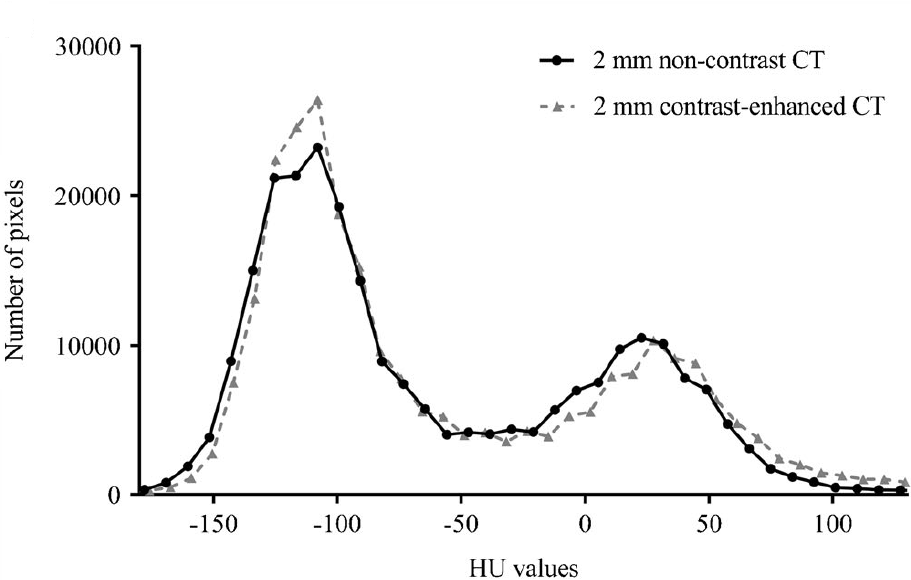
\includegraphics[scale=0.65]{Immagini/fuchs_contrasto2.png}\quad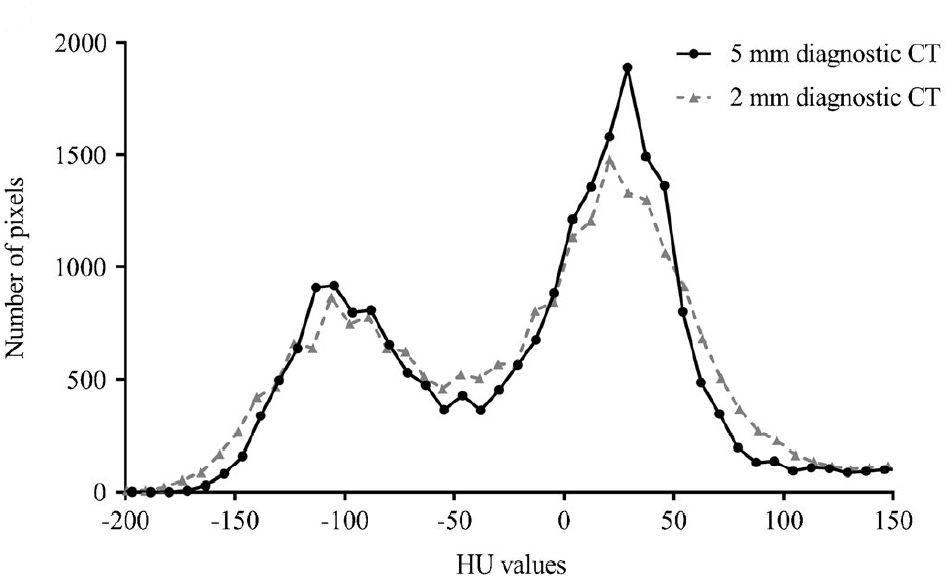
\includegraphics[scale=0.65]{Immagini/fuchs_spessore2.png}
\caption{\label{fig:fuchs_2} \textit{Istogrammi delle immagini TC che mostrano il numero di pixel in funzione delle unità Hounsfield per acquisizioni di slice di $2\,\mathrm{mm}$ con e senza contrasto (immagine di sinistra) e per acquisizioni senza contrasto di slice di $2$ e $5\,\mathrm{mm}$. Si può notare: nell'immagine di sinistra, un numero maggiore di pixel nell'intervallo compreso tra $-120$ e $-100\,\mathrm{HU}$ (tessuto adiposo) per le acquisizioni contrast-enhanced rispetto alle acquisizioni unenhanced; nell'immagine di destra, un numero maggiore di pixel nell'intervallo compreso tra $0$ e $50\,\mathrm{HU}$ (tessuto adiposo e muscolare) per le acquisizioni di slice di $5\,\mathrm{mm}$ rispetto a quelle di $2\,\mathrm{mm}$. Fonte:} \cite{Fuchs2018}.}
\end{figure}

Un altro studio in cui vengono comparate la massa e la densità di muscolo scheletrico nelle differenti fasi di azione del mezzo di contrasto è quello svolto da van Vugt \textit{et al.} \cite{vanVugt2018}. Il \textit{data set} è costituito da TC di 50 pazienti con cancro o in attesa di trapianto di fegato, classificati in quattro categorie mediante il BMI (sottopeso, normopeso, sovrappeso e obesi). Per l’acquisizione di tutte le TC è stato seguito un protocollo standard pianificato in modo da poter distinguere tre fasi durante lo svolgimento delle indagini diagnostiche. Le fasi sono le seguenti: fase \textit{unenhanced} (mezzo di contrasto non ancora somministrato), fase arteriosa e fase venosa portale. Innanzitutto, si esegue una TC senza contrasto, poi viene iniettato il mezzo di contrasto IV, in quantità variabile in base al peso del paziente (minore o maggiore di 80\,kg). 30-35\,s dopo l’iniezione del contrasto IV inizia la fase arteriosa, che consente di vedere lesioni ipervascolarizzate da rami dell'arteria epatica; alla fase arteriosa subentra la fase venosa portale, circa 70\,s dopo l’infusione del contrasto, in cui è possibile valutare quali lesioni sono vascolarizzate dai rami della vena porta \cite{passariello}, un sistema vascolare che ha il compito di convogliare al fegato il sangue proveniente dal tratto gastrointestinale, dal pancreas e dalla milza \cite{porta}. L’inizio della fase arteriosa è stato determinato ponendo una regione d’interesse nell'aorta addominale superiore: l’inizio dell'acquisizione è stato impostato per avvenire 15\,s dopo il raggiungimento di 100\,HU in quella zona. Lo spessore delle \textit{slice} è di 3\,mm in tutte le fasi. La CSMA è stata misurata all'altezza della vertebra L3 in tutte le fasi mediante un software di segmentazione semiautomatica, con il solito intervallo nella scala Hounsfield tra $-30$ e 150\,HU. Dividendo la CSMA espressa in centimetri quadrati per l’altezza del paziente al quadrato espressa in metri quadrati, è stato calcolato l’indice di muscolo scheletrico (SMI). La coorte di pazienti era composta per il 46\% da uomini e per il 54\% da donne; inoltre, il 38\% dei pazienti era sovrappeso e l’8\% obeso. Al variare delle fasi è stato osservato un cambiamento nell’SMI, che è risultato essere $(42,5 \pm 9,9)\,\text{cm}^2/\text{m}^2$ nella fase \textit{unenhanced} (prima della somministrazione del contrasto IV), $(42,8 \pm 9,9)\,\text{cm}^2/\text{m}^2$ nella fase arteriosa e $(43,6 \pm 9,9)\,\text{cm}^2/\text{m}^2$ nella fase venosa portale. Una variazione significativa è stata rilevata anche nella SMD, corrispondente a $(30,9 \pm 8,0)$\,HU nella fase \textit{unenhanced}, a $(38,0 \pm 9,9)$\,HU nella fase arteriosa e a $(38,7 \pm 9,2)$\,HU nella fase venosa portale. I dati sulle variazioni di SMI e SMD sono riportati nella \figref{fig:vanVugt_sm}, mentre le differenze tra le diverse fasi sono espresse in forma di grafici di Bland-Altman nelle figure \ref{fig:vanVugt_smiba} e \ref{fig:vanVugt_smdba}. In base alle misure effettuate, secondo le soglie definite in letteratura, è risultato avere bassa SMD durante la fase \textit{unenhanced} l’80\% dei pazienti, durante la fase arteriosa il 50\% e durante la fase venosa portale il 38\%.
\begin{figure}[htp]
\centering
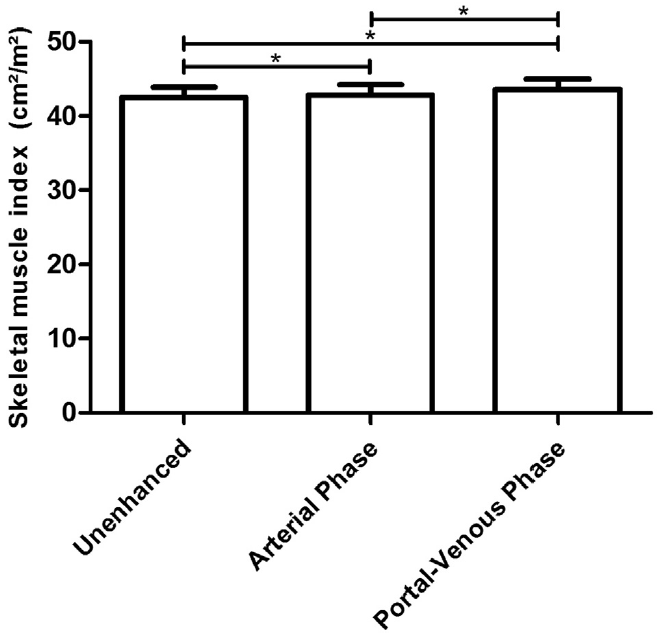
\includegraphics[scale=0.55]{Immagini/vanVugt_smi.png}\quad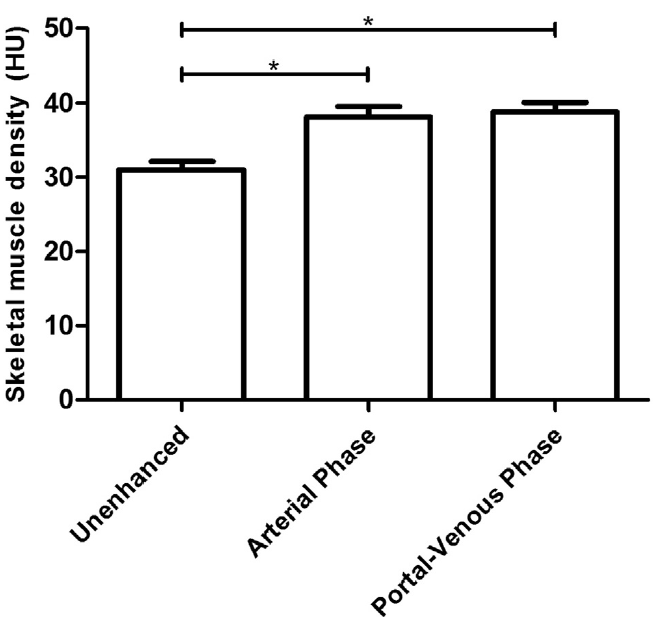
\includegraphics[scale=0.55]{Immagini/vanVugt_smd.png} \vspace{-25pt}
\caption{\label{fig:vanVugt_sm} \textit{Istogrammi di indice di muscolo scheletrico medio (immagine di sinistra) e densità di muscolo scheletrico media (immagine di destra) per fase di contrasto. Le barre di errore rappresentano la deviazione standard della media. Gli asterischi indicano differenze statisticamente significative tra i valori calcolati nelle varie fasi. Fonte:} \cite{vanVugt2018}.}
\end{figure}

\vspace{-5pt}Dalla comparazione delle CSMA è risultata, nella fase \textit{unenhanced}, una percentuale di pazienti sarcopenici sul totale del 44\%, che scende al 42\% nella fase arteriosa e risale al 48\% nella fase venosa portale. La quantità di mezzo di contrasto iniettato in ciascun paziente in base alla sua massa corporea non ha dimostrato nessuna correlazione con la SMD. Sebbene la dipendenza della massa muscolare scheletrica dalla fase sia stata trovata e sia statisticamente significativa, clinicamente il dato importante è quello sulla densità muscolare scheletrica, in quanto maggiormente legato alla diagnosi e alla valutazione del grado di sarcopenia e anche perché correlato al grado di infiltrazioni lipidiche all'interno dei muscoli scheletrici. Nonostante ciò, una massa muscolare scheletrica ridotta è associata a una maggiore tossicità delle terapie antitumorali, dunque è anch'essa importante in fase di definizione e aggiornamento dei piani terapeutici chemioterapici. Gli autori dello studio concludono sottolineando i vantaggi, per una maggiore coerenza e comparabilità tra lavori diversi, di utilizzare preferibilmente TC in fase venosa portale, poiché questo è il tipo di indagine eseguito più spesso per i pazienti malati di cancro; un altro consiglio è di riportare quantomeno la fase in cui vengono acquisite le TC utilizzate.

\begin{figure}[htp]
\centering
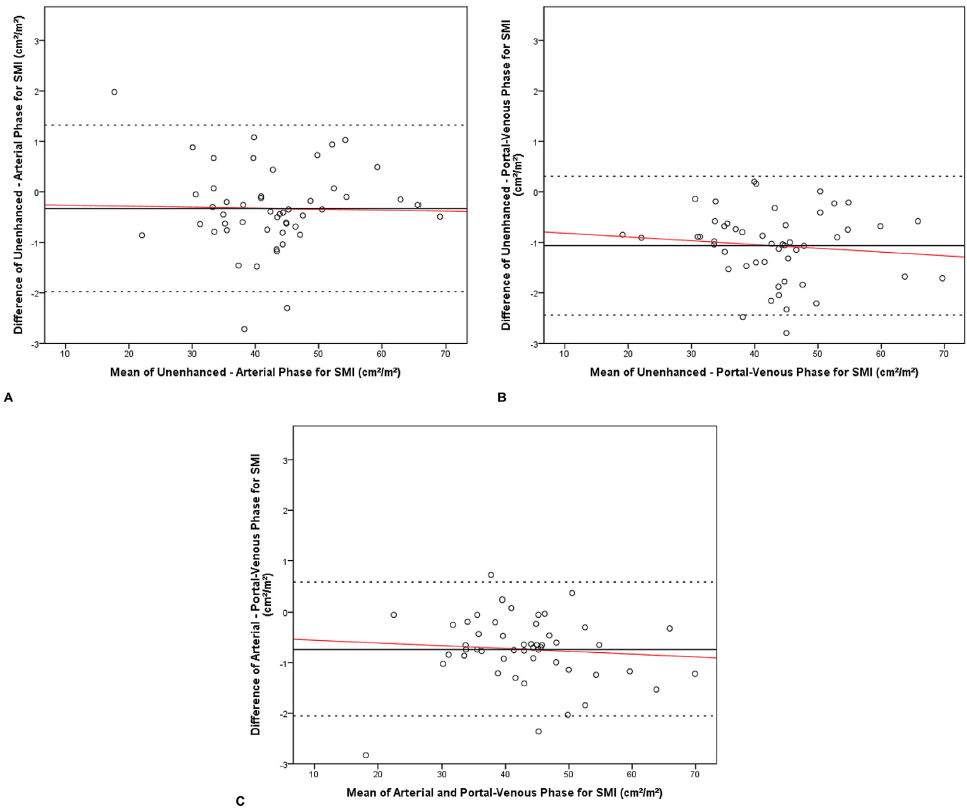
\includegraphics[scale=0.77]{Immagini/vanVugt_smiba.png}
\caption{\label{fig:vanVugt_smiba} \textit{Grafici di Bland-Altman dell'indice di muscolo scheletrico (SMI) per il confronto di: fase unenhanced e fase arteriosa (A), fase unenhanced e fase venosa portale (B) e fase arteriosa e fase venosa portale (C). La linea nera continua rappresenta la differenza media, le linee tratteggiate costituiscono i limiti di concordanza e la linea rossa è la retta di regressione. Fonte:} \cite{vanVugt2018}.}
\end{figure}
\begin{figure}[htp]
\centering
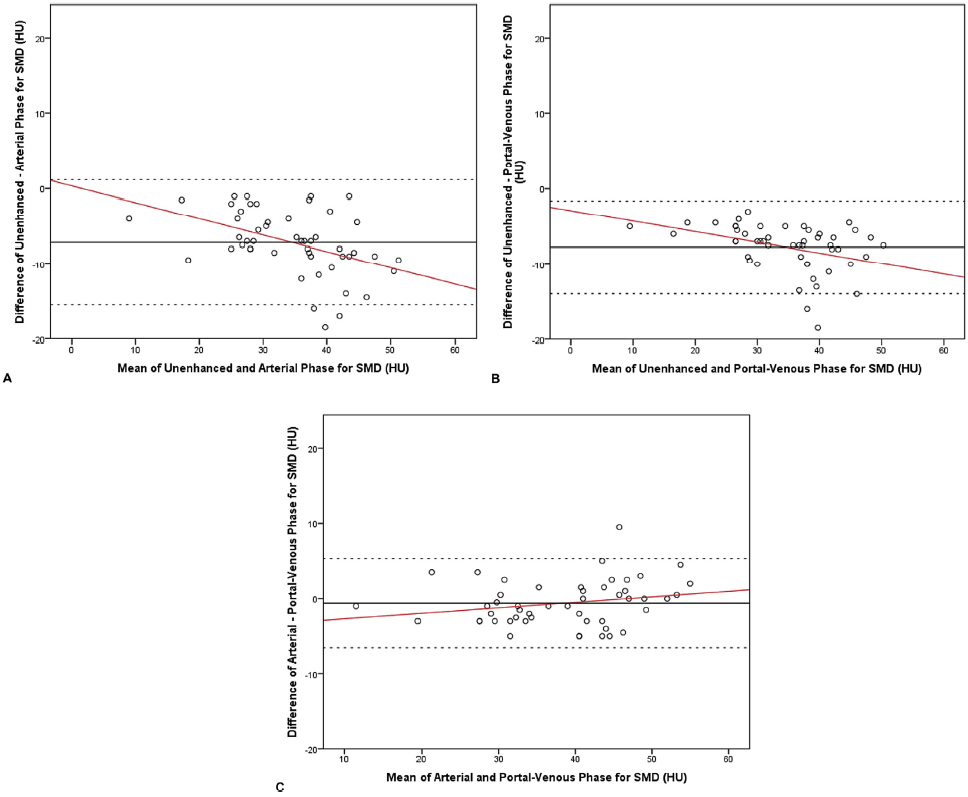
\includegraphics[scale=0.77]{Immagini/vanVugt_smdba.png}
\caption{\label{fig:vanVugt_smdba} \textit{Grafici di Bland-Altman della densità di muscolo scheletrico (SMD) per il confronto di: fase unenhanced e fase arteriosa (A), fase unenhanced e fase venosa portale (B) e fase arteriosa e fase venosa portale (C). La linea nera continua rappresenta la differenza media, le linee tratteggiate costituiscono i limiti di concordanza e la linea rossa è la retta di regressione. Fonte:} \cite{vanVugt2018}.}
\end{figure}

Nei due studi precedenti trova conferma la sospetta necessità di tenere in considerazione il mezzo di contrasto durante lo sviluppo di un software per la segmentazione automatica, a causa delle differenze sostanziali fra i dati ottenuti senza mezzo di contrasto e quelli ottenuti con contrasto IV nelle diverse fasi. Sulla base dei risultati trovati per il tessuto muscolare, ci si potrebbe aspettare risultati analoghi anche per il tessuto adiposo, importante quanto il primo nell'ambito della segmentazione e dei risvolti clinici.
Uno studio analogo a \cite{Fuchs2018}, ma che analizza oltre all'effetto dello spessore delle \textit{slice} e del mezzo di contrasto sui muscoli, anche quello sul tessuto adiposo, è stato realizzato da Morsbach \textit{et al.} \cite{Morsbach2019} su una coorte di 20 pazienti (13 uomini e 7 donne) di età compresa fra 40 e 87 anni, BMI medio di 21,2\,kg/$\text{cm}^2$, con sospetto carcinoma epatocellulare. Il \textit{data set} è costituito da una TC perfusionale per ciascun paziente, con almeno 4 serie acquisite senza mezzo di contrasto e inclusive di una scansione dell'addome ad altezza L3. In una TC di perfusione vengono eseguite delle scansioni a intervalli di 1,5-3\,s che danno luogo a delle serie mirate allo studio del flusso del mezzo di contrasto nei vasi sanguigni, in modo da fornire informazioni sulla vascolarizzazione di un eventuale  tumore. La scansione inizia qualche secondo prima che il mezzo di contrasto si sia diffuso per acquisire anche serie senza mezzo di contrasto. Per la valutazione dell'effetto del mezzo di contrasto sono state ricostruite 18 immagini a livello di L3 da 18 serie, di cui 4 in fase \textit{unenhanced}, 12 in fase arteriosa e 2 in fase venosa portale iniziale; le immagini sono state ricostruite a partire da \textit{slice} dello spessore di 5\,mm. Per valutare l’effetto dello spessore delle \textit{slice} sono state considerate immagini ad altezza L3 da \textit{slice} dello spessore di 2, 3, 4, 5 e 10\,mm, ricostruite dalle 4 serie acquisite durante la fase \textit{unenhanced}. Le immagini sono state segmentate manualmente da un radiologo, sono state calcolate CSA e attenuazione media (da cui si ricava la densità) di ogni tipo di tessuto e anche SMI, indice di tessuto adiposo e superficie di muscolo steatosico (muscolo infiltrato da tessuto adiposo).

Per quanto riguarda la dipendenza dal mezzo di contrasto, è stato rilevato un incremento di SMI con il progredire delle fasi del contrasto (2,8\% di variazione tra l’ultima serie e la prima) e una diminuzione di superficie di muscolo steatosico ($-13,8\%$) e dell'indice di tessuto adiposo ($-6,5\%$). Altri due parametri da segnalare sono l’attenuazione muscolare media, che presenta un incremento del 20\%, passando da 30\,HU nella fase \textit{unenhanced} a 36\,HU nella fase venosa portale, e l’attenuazione adiposa media, con un incremento di circa il 3,3\%, da $-90$\,HU a $-87$\,HU. Riguardo all'effetto dello spessore delle \textit{slice} sono stati trovati incrementi medi dell’1,9\% per l’SMI, del 3,3\% per la superficie muscolare steatosica e dell’1,5\% per l’indice di tessuto adiposo. Nessuna dipendenza è stata trovata in relazione all'attuazione muscolare, mentre per l’attenuazione adiposa è stato rilevato un incremento del 5,5\%.

Nel significativo aumento dell'attenuazione muscolare in relazione alle fasi del contrasto, trovano conferma gli errori metodologici evidenziati negli studi precedenti, che portano a una sovrastima della CSMA e della stessa attenuazione muscolare; gli autori sottolineano la necessità di un protocollo standardizzato per la valutazione della composizione corporea mediante TC. Similmente a quanto riportato dal gruppo di lavoro di Fuchs in \cite{Fuchs2018}, anche in questo studio si trovano delle dipendenze significative di tutti i parametri dallo spessore delle \textit{slice} tranne, sorprendentemente, per quanto riguarda l’attenuazione muscolare.

Un lavoro più specifico sulla dipendenza della segmentazione del tessuto adiposo dai parametri di acquisizione è quello presentato da Troschel \textit{et al.} \cite{Troschel2021}, che ha l'obiettivo di stimare l’influenza del contrasto IV e dello spessore delle \textit{slice} su CSA e attenuazione media di tessuto adiposo sottocutaneo (SAT), viscerale (VAT) e intermuscolare (IMAT). Il \textit{data set} consiste di immagini ottenute con tre tipi di tecniche: \textit{computed tomography angiography} (CTA), \textit{dual-energy CT} (DECT)%
\footnote{La DECT è una tecnica che utilizza due fasci di raggi X di diversa energia, in modo da poter identificare meglio sostanze diverse. Ciò è reso possibile dal fatto che ciascun elemento chimico è caratterizzato da una propria energia di legame della \textit{shell} K, cioè la \textit{shell} più interna di un atomo; c’è più probabilità che un fotone X venga assorbito, generando effetto fotoelettrico, se questo ha energia simile all'energia di legame della \textit{shell} K. L’aumento della probabilità di assorbimento si riflette anche sull'attenuazione di un dato elemento chimico, che sarà maggiore se il fascio utilizzato possiede quella specifica energia che massimizza la probabilità di effetto fotoelettrico. L’utilizzo della DECT, dunque, è principalmente quello di distinguere alcuni elementi con un’energia di legame della \textit{shell} K maggiore di quella dei tessuti circostanti: per esempio può essere utilizzata per distinguere il calcio o lo iodio dai tessuti molli. Poiché la probabilità di osservare l’effetto fotoelettrico prevale per gli elementi con alto numero atomico (per numeri atomici bassi prevale l’effetto Compton), la DECT funziona bene solo per distinguere elementi più pesanti di quelli che costituiscono i tessuti circostanti. Fonte: \cite{Coursey2010}.}
e PET/TC. Dalle scansioni TC ottenute con queste tre tecniche sono state estratte 139 coppie di immagini assiali al livello della vertebra L3; le immagini costituenti ciascuna coppia differiscono l’una dall'altra solo per uno dei seguenti parametri: utilizzo del mezzo di contrasto, spessore delle \textit{slice}, dose somministrata e potenziale del tubo. Ciascuna coppia è stata ottenuta dallo stesso paziente durante la stessa sessione di acquisizione con lo stesso scanner. Tralasciando gli ultimi due parametri, che sebbene siano rilevanti avrebbero bisogno di una trattazione molto più lunga e dettagliata, le implicazioni del contrasto IV sono state analizzate su 37 acquisizioni CTA mediante il confronto tra fase \textit{unenhanced} e fase venosa portale; gli effetti dello spessore delle \textit{slice} sono stati valutati su 34 acquisizioni PET/TC mediante il confronto fra immagini acquisite con spessore di 5\,mm in fase \textit{unenhanced} e le stesse immagini ricostruite da \textit{slice} dallo spessore di 2\,mm.

La segmentazione dei tessuti a L3 è stata realizzata mediante un software di segmentazione semiautomatica, con soglie tra $-190$ e $-30$\,HU per il tessuto adiposo e tra $-29$ e 150\,HU per il tessuto muscolare. Sono state rilevate riduzioni significative nelle CSA di SAT ($-0,4\%$) e IMAT ($-9,3\%$) come effetto del contrasto IV; una riduzione della CSA è stata osservata anche per il VAT ($-2,0\%$) ma questa non è risultata statisticamente significativa. Allo stesso tempo sono stati trovati aumenti significativi dell'attenuazione media per SAT (0,8\%), VAT (1,7\%) e IMAT (0,8\%). L’utilizzo di \textit{slice} più sottili ha comportato aumenti significativi delle CSA di VAT (3,0\%) e IMAT (17,3\%) e una decrescita non significativa per il SAT ($-0,2\%$). Contemporaneamente, sono stati osservati decrementi significativi dell'attenuazione media per SAT ($-2,0\%$), VAT ($-2,4\%$) e IMAT ($-5,4\%$).

I risultati confermano quanto già riportato dal gruppo di Morsbach in \cite{Morsbach2019}, aggiungendo informazioni anche su SAT e IMAT; trovano conferma anche i dati ottenuti dallo studio della dipendenza dallo spessore delle \textit{slice} per tutti i tipi di tessuto adiposo. La differenziazione tra questi tessuti nasce dalle loro differenti genesi e implicazioni: grandi CSA di SAT e VAT sono correlate con stati di obesità \cite{Troschel2020, Troschel2021}, con il VAT molto più pericoloso perché considerato uno dei principali fattori di rischio per eventi avversi e malattie cardiovascolari; l’IMAT invece è indice di scarsa qualità muscolare \cite{Reinders2015, Troschel2021} e insulinoresistenza \cite{Goodpaster2000, Troschel2021}. D’altra parte, le CSA di SAT e VAT sono associate a una maggiore probabilità di sopravvivenza in pazienti affetti da carcinoma epatocellulare \cite{Fujiwara2015, Troschel2021} e a una maggiore \textit{progression-free survival} in pazienti colpiti da cancro al polmone \cite{Nattenmüller2017, Troschel2021}.

In \cite{Perez2021} viene svolto un lavoro di correzione degli effetti che il contrasto IV ha sui risultati delle scansioni TC, rispetto proprio alle misure effettuate da software di segmentazione automatica. La coorte analizzata consta di 1211 pazienti, di cui sono state acquisite, prima dell'iniezione del contrasto IV, serie di TC addominali tra le vertebre T12-L4. Riguardo alla somministrazione del mezzo di contrasto, questa è avvenuta in due fasi: una prima iniezione è stata effettuata per l’acquisizione della fase arteriosa, la seconda per l’acquisizione della fase parenchimale, cioè la fase in cui l’organo, il rene nello specifico, mostra il contrasto maggiore. Le serie sono state acquisite in \textit{slice} di 5\,mm e ricostruite successivamente in \textit{slice} di 3\,mm di spessore. L’effetto del mezzo di contrasto è stato valutato confrontando le misurazioni effettuate nella fase \textit{unenhanced} con quelle effettuate nella fase parenchimale, utilizzando il livello L3 per misurare la superficie e l’attenuazione media della parete muscolare addominale, mentre al livello L1 sono stati misurati l’attenuazione trabecolare ossea e il rapporto tra grasso viscerale e sottocutaneo (VSR).

Nella fase parenchimale sono state registrate diminuzioni di superfici (rispetto alla fase \textit{unenhanced}) sia per il grasso viscerale sia per quello sottocutaneo, rispettivamente del 25,4\% e del 9,4\%; i coefficienti di correlazione lineare $r^2$ sono risultati pari a 0,96 e 0,98, rispettivamente. Il VSR è passato da $ 0,87 \pm 0,73 $ nella fase \textit{unenhanced} a $ 0,74 \pm 0,68 $ nella fase parenchimale, con la deviazione standard presa come incertezza; tra le due fasi si osserva, quindi, una decrescita del VSR del 17\% e un coefficiente di correlazione $r^2$ pari a 0,97. In accordo con la tendenza registrata negli studi precedentemente riportati, anche in questo lavoro si riscontra un aumento della superficie di tessuto muscolare, del 2,4\% in media con un coefficiente di correlazione pari a 0,93. Allo stesso tempo, come ci si aspettava, è stato rilevato un aumento dell'attenuazione muscolare media del 77,3\%, accompagnato da un grado di correlazione meno pronunciato, testimoniato da un $r^2 = 0,75$. Infine c’è da segnalare l’aumento dell'attenuazione trabecolare del 15,8\% con $r^2 = 0,72$. Le correlazioni menzionate nel presente capoverso sono riportate nei grafici di \figref{fig:perez_correlazioni}.

\begin{figure}[htp]
\centering
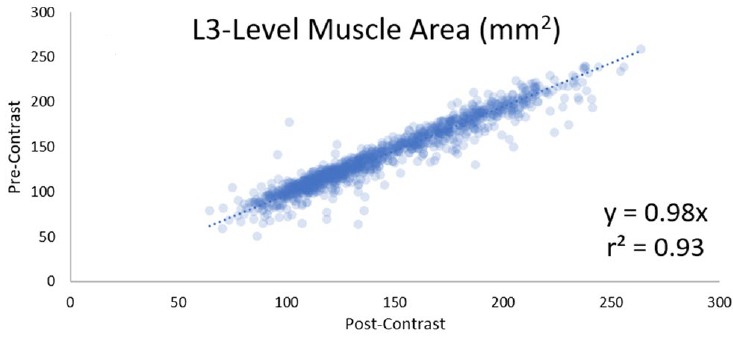
\includegraphics[scale=0.49]{Immagini/perez_areamuscolo.png}\quad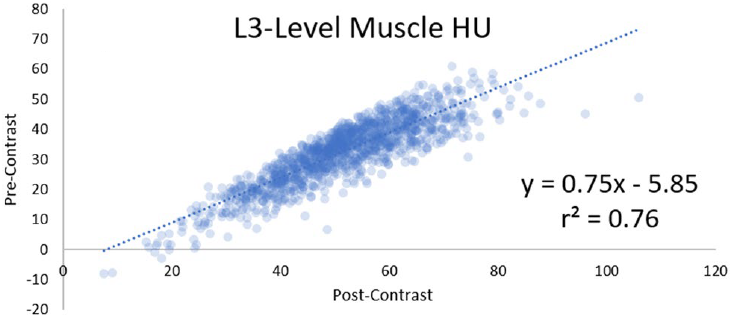
\includegraphics[scale=0.49]{Immagini/perez_attenuazionemuscolo.png}\quad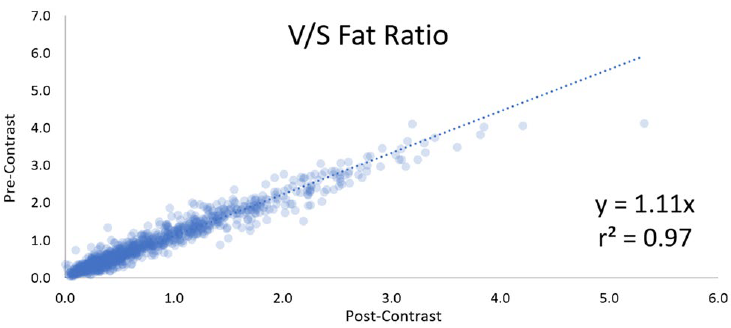
\includegraphics[scale=0.49]{Immagini/perez_vsr.png}\quad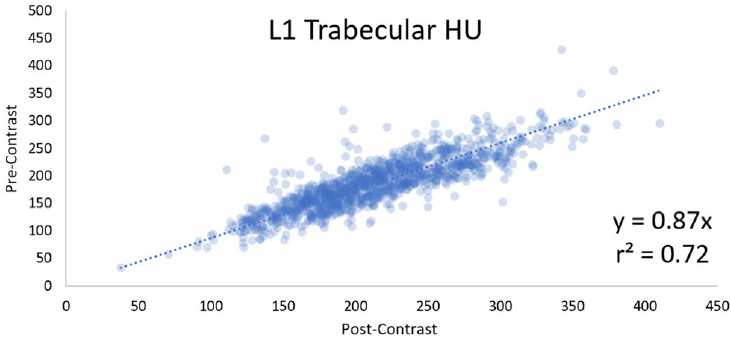
\includegraphics[scale=0.49]{Immagini/perez_trabecole.png}
\caption{\label{fig:perez_correlazioni} \textit{Grafici precontrasto vs postcontrasto di superficie e attenuazione muscolare, misurate a L3, e di VSR e attenuazione trabecolare, misurati a L1. Fonte:} \cite{Perez2021}.}
\end{figure}

L’algoritmo di segmentazione ha commesso alcuni errori con maggiore frequenza di altri nel segmentare le immagini, tra cui parti mancanti durante la segmentazione del muscolo, cattiva segmentazione del grasso in prossimità della fascia muscolare addominale ed erroneo posizionamento della regione d’interesse all'interno della vertebra, con inclusione anche dell'osso corticale (la parte più esterna dell'osso, che va esclusa se si vuole misurare l’attenuazione dell'osso trabecolare); esempi di questi errori sono riportati in \figref{fig:perez_errori}. La soluzione proposta dagli autori è semplicemente quella di utilizzare come \virgolette{ponte} tra TC senza e con contrasto le regressioni lineari trovate, sebbene essi raccomandino anche controlli di validità della segmentazione proposta dall'algoritmo da parte del personale medico preposto.

\begin{figure}[htp]
\centering
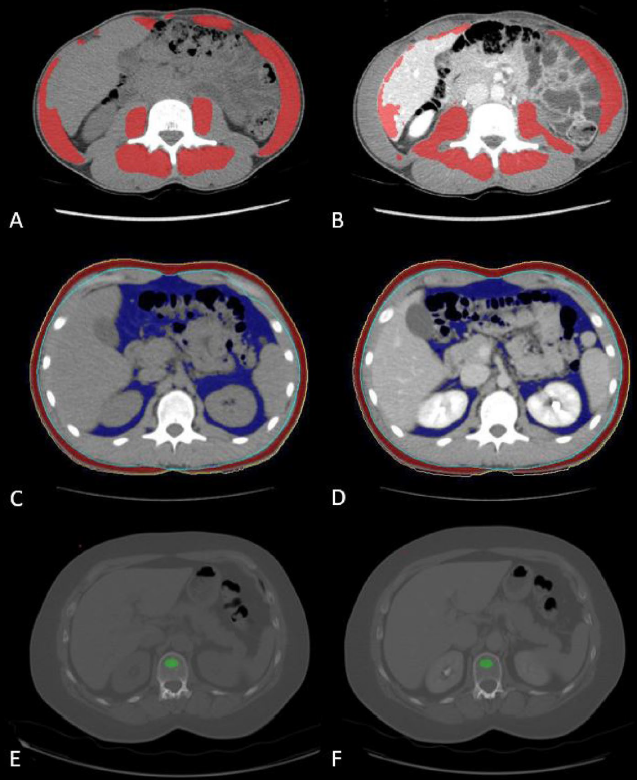
\includegraphics[scale=0.9]{Immagini/perez_errori.png}
\caption{\label{fig:perez_errori} \textit{In alto: segmentazioni precontrasto (A) e postcontrasto (B) di muscolo scheletrico, con evidenti errori di segmentazione in entrambe le immagini. In mezzo: segmentazioni precontrasto (C) e postcontrasto (D) di grasso viscerale (in blu) e sottocutaneo (in rosso); nell'immagine C non si riscontrano errori, mentre nell'immagine D alcune porzioni di grasso viscerale non vengono più riconosciute a causa della differenza nell'attenuazione provocata dall'effetto del mezzo di contrasto. In basso: segmentazioni precontrasto (E) e postcontrasto (F) di osso trabecolare in L1, dove però nell'immagine E la regione di interesse è troppo grande e include anche una parte di osso corticale. Fonte:} \cite{Perez2021}.}
\end{figure}

\section{L'approccio 3D alla segmentazione TC}
Tutti gli studi finora riportati assumono le misure dei tessuti eseguite nella regione T11-L5, e soprattutto per la vertebra L3, come affidabili per la stima della composizione corporea; ciò è dovuto ai numerosi studi che negli ultimi venti anni hanno dimostrato la correlazione fra le misure \textit{single slice} 2D e le misure volumetriche 3D. D’altra parte, sebbene le misure effettuate in 2D rappresentino un buon indicatore per gruppi di studio, ciò non implica che queste stesse misure debbano avere valore prognostico per i singoli pazienti \cite{Ma2021}. In uno studio del 2004 \cite{Shen2004}, Shen \textit{et al.} hanno dimostrato, oltre alla correlazione tra misure 2D e 3D, che considerare diverse \textit{slice} trasversali piuttosto che una sola fornisce una correlazione maggiore. Questa sembra essere l’unica strada percorribile per aumentare l’accuratezza delle misure, dato che l’equazione di regressione trovata in \cite{Shen2004} non può essere generalizzata a tutte le fasce d’età e fra altre categorie di pazienti. Questi dettagli ed altri, che negli studi di gruppo possono essere trascurati per effetto del campione numeroso che si va ad analizzare, possono invece portare ad errori di valutazione per i singoli pazienti, per cui di conseguenza è necessario cercare di condurre analisi il più possibile precise.

Ci sono anche situazioni in cui effettuare misure \textit{single slice} risulta critico, come stimare i volumi e valutare le funzionalità degli organi interni. Per questo motivo, in \cite{Ma2021} viene sottolineata la necessità di sviluppare modelli per il calcolo della composizione corporea non più mediante l’approccio \textit{single slice} ma attraverso misure 3D, possibilmente riguardanti tutto il corpo. Le segmentazioni utilizzate come \textit{ground truth} per l’algoritmo sono state realizzate con un software di segmentazione semiautomatica da degli anatomisti, che hanno preso in considerazione quattro tessuti: muscolo scheletrico (SM), osso, tessuto adiposo sottocutaneo (SAT) e tessuto adiposo viscerale (VAT). Dal \textit{data set} sono state estratte 21 segmentazioni divise in base alla vertebra di riferimento: 4 dalle vertebre cervicali C4-C7, 12 dalle vertebre toraciche T1-T12 e 5 dalle vertebre lombari L1-L5. La segmentazione automatica è stata eseguita mediante la piattaforma DAFS (\textit{Voronoi Health Analytics} \cite{voronoi}), le cui analisi hanno ottenuto dei coefficienti di Dice di 0,980 per l’osso, 0,974 per l’SM, 0,986 per il SAT e 0,960 per il VAT, come si può vedere nella \figref{fig:ma_dice}. In \figref{fig:ma_3d} è riportato un esempio di segmentazione automatica effettuato sulla piattaforma DAFS di alcune immagini TC, insieme alla ricostruzione tridimensionale delle segmentazioni.
\begin{figure}[htp]
\centering
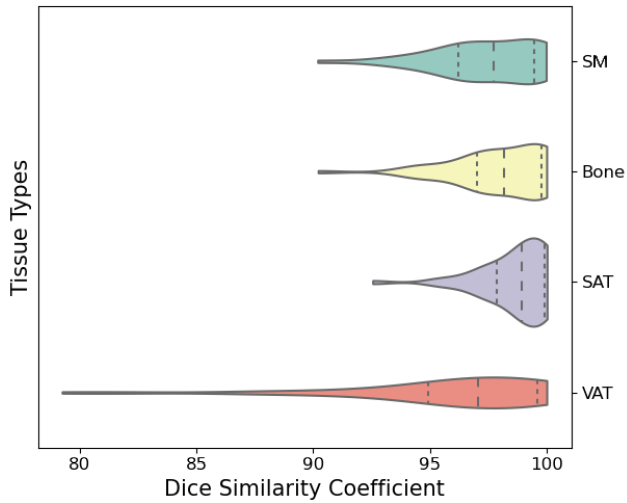
\includegraphics[scale=0.75]{Immagini/ma_dice.png}
\caption{\label{fig:ma_dice} \textit{Diagrammi a violino dei coefficienti di Dice per ogni tessuto. Fonte:} \cite{Ma2021}.}
\end{figure}
\begin{figure}[htp]
\centering
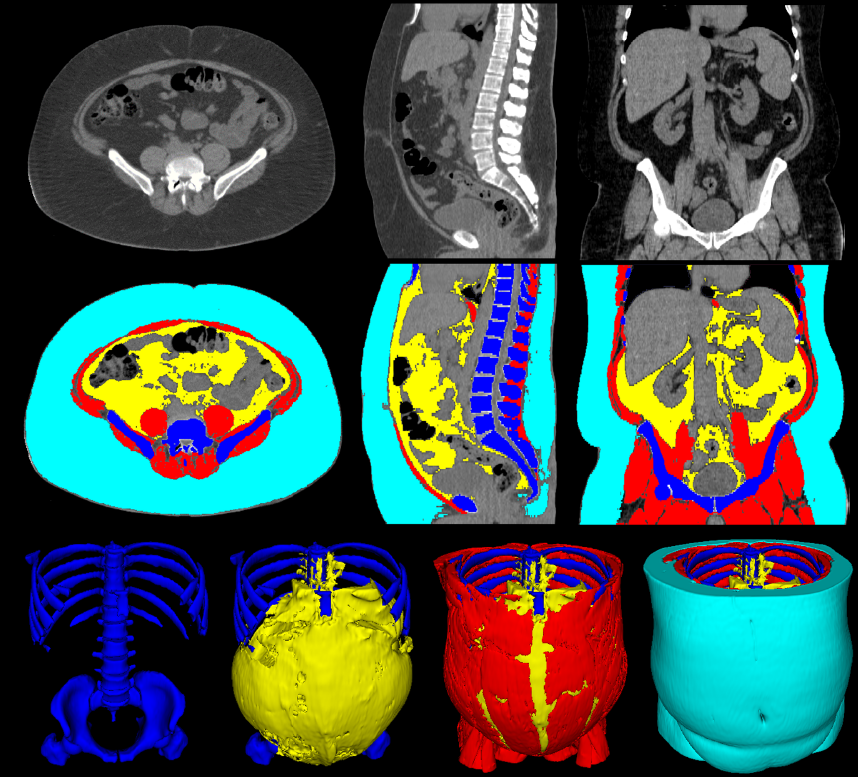
\includegraphics[scale=0.8]{Immagini/ma_3d.png}
\caption{\label{fig:ma_3d} \textit{Da sinistra a destra, visioni assiali, sagittali e coronali di: in alto, immagini TC originali; in mezzo, segmentazioni delle immagini TC di grasso viscerale (giallo), grasso sottocutaneo (azzurro), muscolo (rosso) e osso (blu); in basso, ricostruzione in tre dimensioni dei tessuti segmentati. Fonte:} \cite{Ma2021}.}
\end{figure}

Nella \figref{fig:ma_vertebre} sono rappresentati i risultati di un’analisi \textit{whole body} in termini di volume e attenuazione media di ogni singolo tessuto, indicizzata verticalmente dalle singole vertebre. Si può vedere come l’attenuazione dei diversi tessuti sia piuttosto costante per tutte le vertebre, ma il dato più interessante è rappresentato dalle distribuzioni del SAT e del VAT, che presentano grosse variabilità nei volumi di tessuto nella regione lombare rispetto al resto del corpo. Questi risultati confermano la rappresentatività della vertebra L3 come indicatore valido per stime di composizione corporea, poiché a questa altezza è possibile valutare le differenze in termini di SAT e VAT tra i vari soggetti; in altre parole, la misura delle superfici trasversali dei tessuti nella regione lombare permette la stratificazione dei pazienti sulla base dei volumi di tessuto adiposo. Nonostante ciò, in generale si conferma la problematica, riportata già in \cite{Shen2004}, della non completa validità dell'approccio \textit{single slice} in casi delicati come la definizione dei piani chemioterapici: i modelli di correlazione superficie-volume, infatti, non garantiscono un'accuratezza tale da poter essere utilizzati in ambito clinico, mentre sono accettabili all'interno di studi epidemiologici.

Per concludere, il gruppo di Ma mette in luce in \cite{Ma2021} le potenzialità e il valore dei dati che si potrebbero ottenere da indagini TC 3D, le quali permettono stime molto più accurate della composizione corporea; d’altro canto, se già la segmentazione di una singola \textit{slice} per TC è un processo lungo, se consideriamo che questo processo deve essere ripetuto per più pazienti, la segmentazione di più di una \textit{slice} per paziente, come richiede l’approccio 3D, diventa praticamente impossibile da portare avanti se non con un algoritmo di segmentazione automatica. La piattaforma DAFS, utilizzata dal gruppo di lavoro di Ma, ha ottenuto degli ottimi risultati in termini di coefficiente di similarità di Dice e ha le potenzialità, secondo gli autori del lavoro, di poter implementare col tempo anche \textit{tool} di subsegmentazione, ad esempio misurando il grasso nelle cavità addominali, ventrali e pelviche e suddividendo il grasso di ognuna di queste regioni in regioni anatomiche più piccole. Un software di segmentazione automatica renderebbe anche possibile la misura delle grandezze degli organi interni menzionate prima, sempre perché renderebbe possibile l’applicazione dell'approccio 3D.
\begin{figure}[htp]
\centering
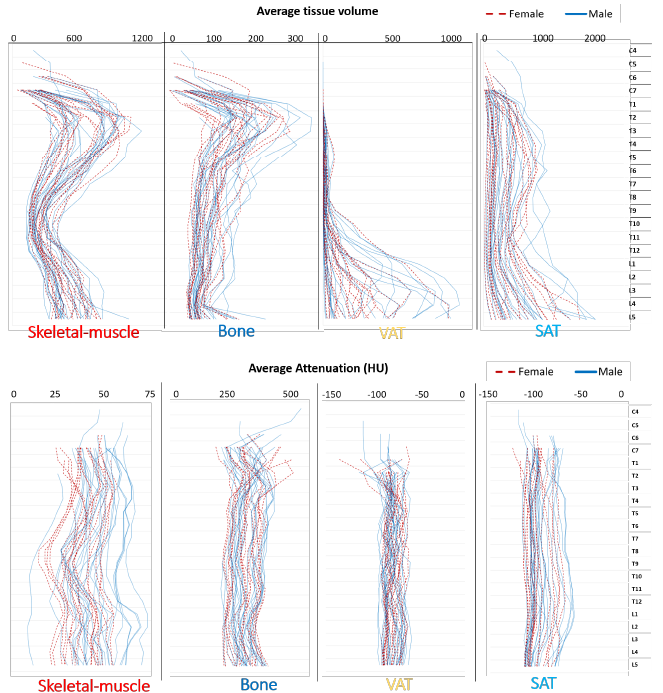
\includegraphics[scale=1.12]{Immagini/ma_vertebre.png}
\caption{\label{fig:ma_vertebre} \textit{Distribuzioni di volumi (in alto) e attenuazioni medie (in basso) per ogni tipo di tessuto e per ogni livello vertebrale. Si può notare un'attenuazione piuttosto costante per tutti i tessuti in entrambi i sessi, mentre i volumi presentano pronunciate variazioni per tutti i tessuti in vertebre diverse, in alcuni casi con differenze importanti anche fra i due sessi. Fonte:} \cite{Ma2021}.}
\end{figure}